The assignment of this report conveyed critizing and accessing system-level Internet of Things components in scientific literature. Because the assigned paper \cite{paper} did not include anything IoT related, we came up with our own idea.
In this section we will provide a short introduction to the Internet of Things and its key features, we will also present our idea and focus on the practicality and entrpreneurial aspect of our idea.

The anatomy of Internet of Things is initiated by a certain event, that is detected and logged by devices that include self-properties \cite{lecture}. This data is then uploaded by a ubiquitous and interoperable network. An analysis of this data can sequentially trigger certain events as a response. The intelligence of these systems lie in the adapting mechanisms that analyse and understand the environment in order to deal with the complex dynamics of a real-world environment.

Internet of Things has already been employed at multiple festivals and initially used as a ticketing solution in 2004 at the SXSW festival in Austin. IoT first introduced itself in the form of wristbands and cut down significantly on gate crashing and lost tickets \cite{thingmagic}. SXSW announced that each tag contained a unique ID code, correlated with personal information availabe by SXSW \cite{sxsw}. Since then it has further been introduced at Coachella and Bonnaroo festivals \cite{coachella} \cite{bonnaroo}. RFID tags now even support cashlesh payments and integration with social networks, allowing people to upload pictures to facebook via the so-called "Live Click Stations"\cite{thingmagic}. It safe to say that the Internet of Things hasn't reached its peak yet concerning these social events and are worth looking into.

The users in our scenario are wearing a wristband containing the specified wireless power receivers. We will add some small features to the wristband to play into current trends concerning Internet of Things and music festivals. By adding a RFID tag into each wristband, users are assigned unique IDs that can provide unique entrance IDs or support cashlesh payments. Figure \ref{fig:iot} displays our choosen chain of interactions considering the Internet of Things as will be discussed afterwards. 

\begin{figure}[h!]
\centering
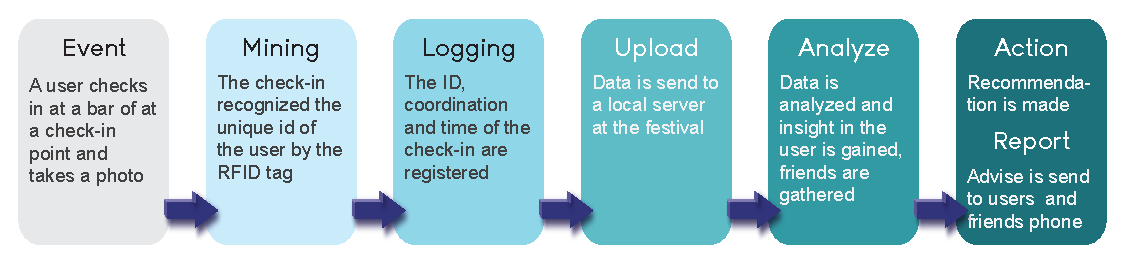
\includegraphics[width=1\textwidth]{IoT.pdf}
\caption{Internet of things chain of actions}
\label{fig:iot}
\end{figure}
%
In this report we want to focus on the fun factor of connecting with friends and strangers. Before arriving at the festival, users are assigned a unique ID when creating an account online. Optionally they can link their accounts with social media or friends and provide some preferences in music. When they arrive at the site and receive their wristbands, their unique IDs are connected with the wristband received. Whenever they charge their wristband at an energy bar or at check in points near every site of interest, their friends that are not near them will receive a message containing their location and if made, an image at the check-in location. Based on certain check-in's at time in the schedule of the festival, the system can recognize their interests (if not already mentioned in their id page online) and provide recommendations.

Our system goes beyond simply assigning a unique ID to a user, it also adds functionality and connects IDs to exchange information. This doesn't just improve the experience of the user, but it gives the organization a better insight into the behavior of their visitors.









